\subsection{UC19 - Autenticazione su \glossario{Piattaforma Riunioni} esterna}
\begin{itemize}
	\item \textbf{Identificativo}: UC19
	\item \textbf{Nome}: Autenticazione su \glossario{Piattaforma Riunioni} esterna
	\item\textbf{Descrizione Grafica}: 
	\begin{center}
		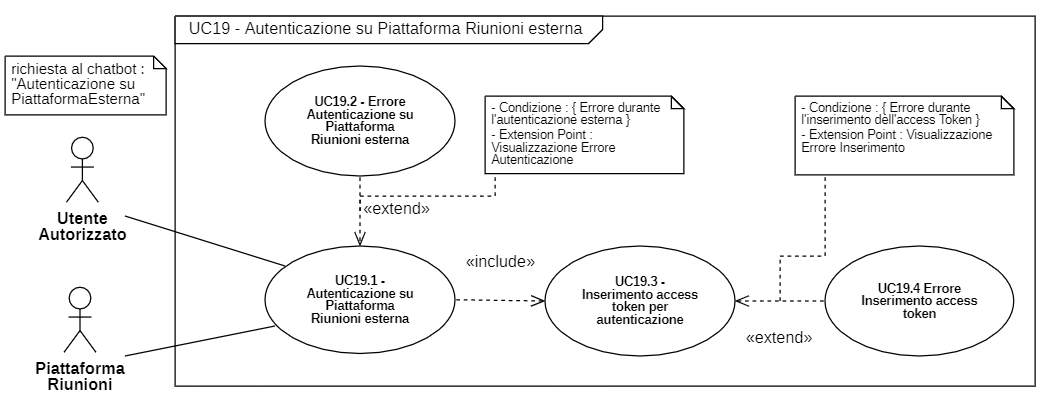
\includegraphics[scale=0.65]{images/UC19.png} 
	\end{center}

	\item \textbf{Attori}
	\begin{itemize} 
		\item \textit{Primari}: Utente autorizzato e non autenticato nella \glossario{Piattaforma Riunioni} esterna
		\item \textit{Secondari}: Piattaforma Riunioni esterna
	\end{itemize}
	\item \textbf{Descrizione}: L'utente vuole eseguire il login su \glossario{Piattaforma Riunioni} esterna.
	\item \textbf{Precondizione}: L'utente non ha un \glossario{access token} necessario per inserire riunioni sull'app esterna.
	\item \textbf{Postcondizione}: L'utente riceve il link per effettuare il login ed ottenere l'\glossario{access token}.
	\item \textbf{Scenario principale}: \begin{enumerate}
		\item Utente deve fare il login (UC19.1) ed il bot fornisce il link per effettuare il login su \glossario{Piattaforma Riunioni} esterna; 
		\item Utente inserisce \glossario{access token} ricevuto dopo aver effettuato il login. (UC19.3)
	\end{enumerate}
\end{itemize}

\subsubsection{UC19.1 - Autenticazione su Piattaforma Riunioni esterna }
\begin{itemize}
	\item \textbf{Identificativo}: UC19.1
	\item \textbf{Nome}: Autenticazione su Piattaforma Riunioni esterna
	\item \textbf{Attori}
	\begin{itemize} 
		\item \textit{Primari}: Utente autorizzato
		\item \textit{Secondari}: Piattaforma Riunioni esterna
	\end{itemize}
	\item \textbf{Descrizione}: L'utente vuole eseguire il login su \glossario{Piattaforma Riunioni} esterna per poter creare riunioni.
	\item \textbf{Precondizione}: L'utente non ha eseguito il login su \glossario{Piattaforma Riunioni} esterna.
	\item \textbf{Postcondizione}: L'utente ha eseguito il login su \glossario{Piattaforma Riunioni} esterna.
	\item \textbf{Scenario principale}: \begin{enumerate}
		\item Utente esegue il login su \glossario{Piattaforma Riunioni} esterna; 
	\end{enumerate}
\end{itemize}

\subsubsection{UC19.2 - Errore Autenticzione su Piattaforma Riunioni esterna}
\begin{itemize}
	\item \textbf{Identificativo}: UC19.2
	\item \textbf{Nome}: Errore Autenticzione su Piattaforma Riunioni esterna
	\item \textbf{Attori}
	\begin{itemize} 
		\item \textit{Primari}: Utente autorizzato
		\item \textit{Secondari}: Piattaforma Riunioni esterna
	\end{itemize}
	\item \textbf{Descrizione}: L'utente vuole eseguire il login su \glossario{Piattaforma Riunioni} esterna ma incontra un errore.
	\item \textbf{Precondizione}: L'utente non ha eseguito il login su \glossario{Piattaforma Riunioni} esterna.
	\item \textbf{Postcondizione}: L'utente non riesce ad eseguire il login su \glossario{Piattaforma Riunioni} esterna ed il bot visualizza l'errore.
	\item \textbf{Scenario principale}: \begin{enumerate}
		\item Chatbot comunica : "Errore nella procedura di autenticazione". 
	\end{enumerate}
\end{itemize}

\subsubsection{UC19.3 - Inserimento \glossario{access token} per autenticazione }
\begin{itemize}
	\item \textbf{Identificativo}: UC19.3
	\item \textbf{Nome}: Inserimento \glossario{access token} per autenticazione
	\item \textbf{Attori}
	\begin{itemize} 
		\item \textit{Primari}: Utente autorizzato
		\item \textit{Secondari}: Nessuno
	\end{itemize}
	\item \textbf{Descrizione}: L'utente vuole eseguire il login su \glossario{Piattaforma Riunioni} esterna.
	\item \textbf{Precondizione}: L'utente ha ottenuto un \glossario{access token} necessario per inserire riunioni su app esterna.
	\item \textbf{Postcondizione}: L'utente inserisce l'\glossario{access token} appena ricevuto.
	\item \textbf{Scenario principale}: \begin{enumerate}
		\item Utente inserisce l'\glossario{access token} ricevuto a seguito del login; 
	\end{enumerate}
\end{itemize}

\subsubsection{UC19.4 - Errore Inserimento access token }
\begin{itemize}
	\item \textbf{Identificativo}: UC19.4
	\item \textbf{Nome}: Errore Inserimento access token
	\item \textbf{Attori}
	\begin{itemize} 
		\item \textit{Primari}: Utente autorizzato
		\item \textit{Secondari}: Nessuno
	\end{itemize}
	\item \textbf{Descrizione}: L'utente vuole eseguire il login su \glossario{Piattaforma Riunioni} esterna ma incontra un errore nell'inserimento dell'access token.
	\item \textbf{Precondizione}: L'utente ha ottenuto un \glossario{access token} necessario per inserire riunioni su app esterna.
	\item \textbf{Postcondizione}: L'utente inserisce l'\glossario{access token} appena ricevuto ma viene notificato con un errore.
	\item \textbf{Scenario principale}: \begin{enumerate}
		\item Utente inserisce l'\glossario{access token} ricevuto a seguito del login; 
		\item Chatbot notifica Utente dell'impossibilità di compiere quest'azione.
	\end{enumerate}
\end{itemize}